\documentclass[12pt]{article}
\usepackage[utf8]{inputenc}
\usepackage{amsmath, amssymb, amsthm}
\usepackage{enumitem}
\usepackage{geometry}
\usepackage{fancyhdr}
\usepackage{pgfplots}
\usepackage{tikz}
\usepackage{float}
\usepackage{graphicx}
\DeclareMathOperator{\Tr}{Tr}
\DeclareMathOperator{\rng}{rng}
\DeclareMathOperator{\norm}{||}
\DeclareMathOperator{\NN}{\mathbb{N}}
\DeclareMathOperator{\ZZ}{\mathbb{Z}}
\DeclareMathOperator{\QQ}{\mathbb{Q}}
\DeclareMathOperator{\RR}{\mathbb{R}}
\DeclareMathOperator{\CC}{\mathbb{C}}

% Page setup
\setlength{\headheight}{15pt}
\geometry{letterpaper, margin=1in}
\setlength{\parindent}{0pt}
\setlength{\parskip}{1em}
\pagestyle{fancy}
\fancyhf{}
\fancyhead[L]{\textbf{Sebastian Griego}}  % Replace with your name
\fancyhead[C]{\textbf{Math Modeling}}  % Replace with your course name
\fancyhead[R]{\textbf{Assignment \#2}}  % Replace with your assignment number
\fancyfoot[C]{\thepage}

\newenvironment{problem}[1]{
    \textbf{Problem #1:}
}{
    \rmfamily \vspace{1em}
}

\newenvironment{solution}{
    \textbf{Solution:}
    
}{
    
    \vspace{2em}
}

\begin{document}

\title{Homework \#2}  % Replace with the homework number
\author{Sebastian Griego}  % Replace with your name

\begin{problem}{5}
    The spruce budworm model
    \[
        \frac{dN(t)}{dt} = r_BN(t) \left( 1 - \frac{N(t)}{K_B} \right) - B\frac{N(t)}{A^2+N(t)^2},
    \]
    can be reduced to the following scaled equation
    \[
        \frac{du}{d\tau} = ru(1-\frac{u}{q}) - \frac{u^2}{1+u^2},
    \]
    Perform the stability analysis and the bifurcation analysis with the parameter \( r \) fixed and the parameter \( q \) as a bifurcation parameter. Also, plot the bifurcation diagram.
\end{problem}

\begin{solution}
    Set \(\frac{du}{d\tau} = 0\) to find the equilibrium points.
    
    \(u^*=0\) is always an equilibrium point.
    
    From class, the other equlibirum happens when
    \[
        \begin{aligned}
            r \left( 1 - \frac{u}{q} \right) &= \frac{u^2}{1+u^2}\\
            g(u) &= h(u)
        \end{aligned}
    \]
    Let \(f(u) = u(g(u) - h(u))\).
    Here are the graphs:
    \begin{figure}[H]
        \centering
        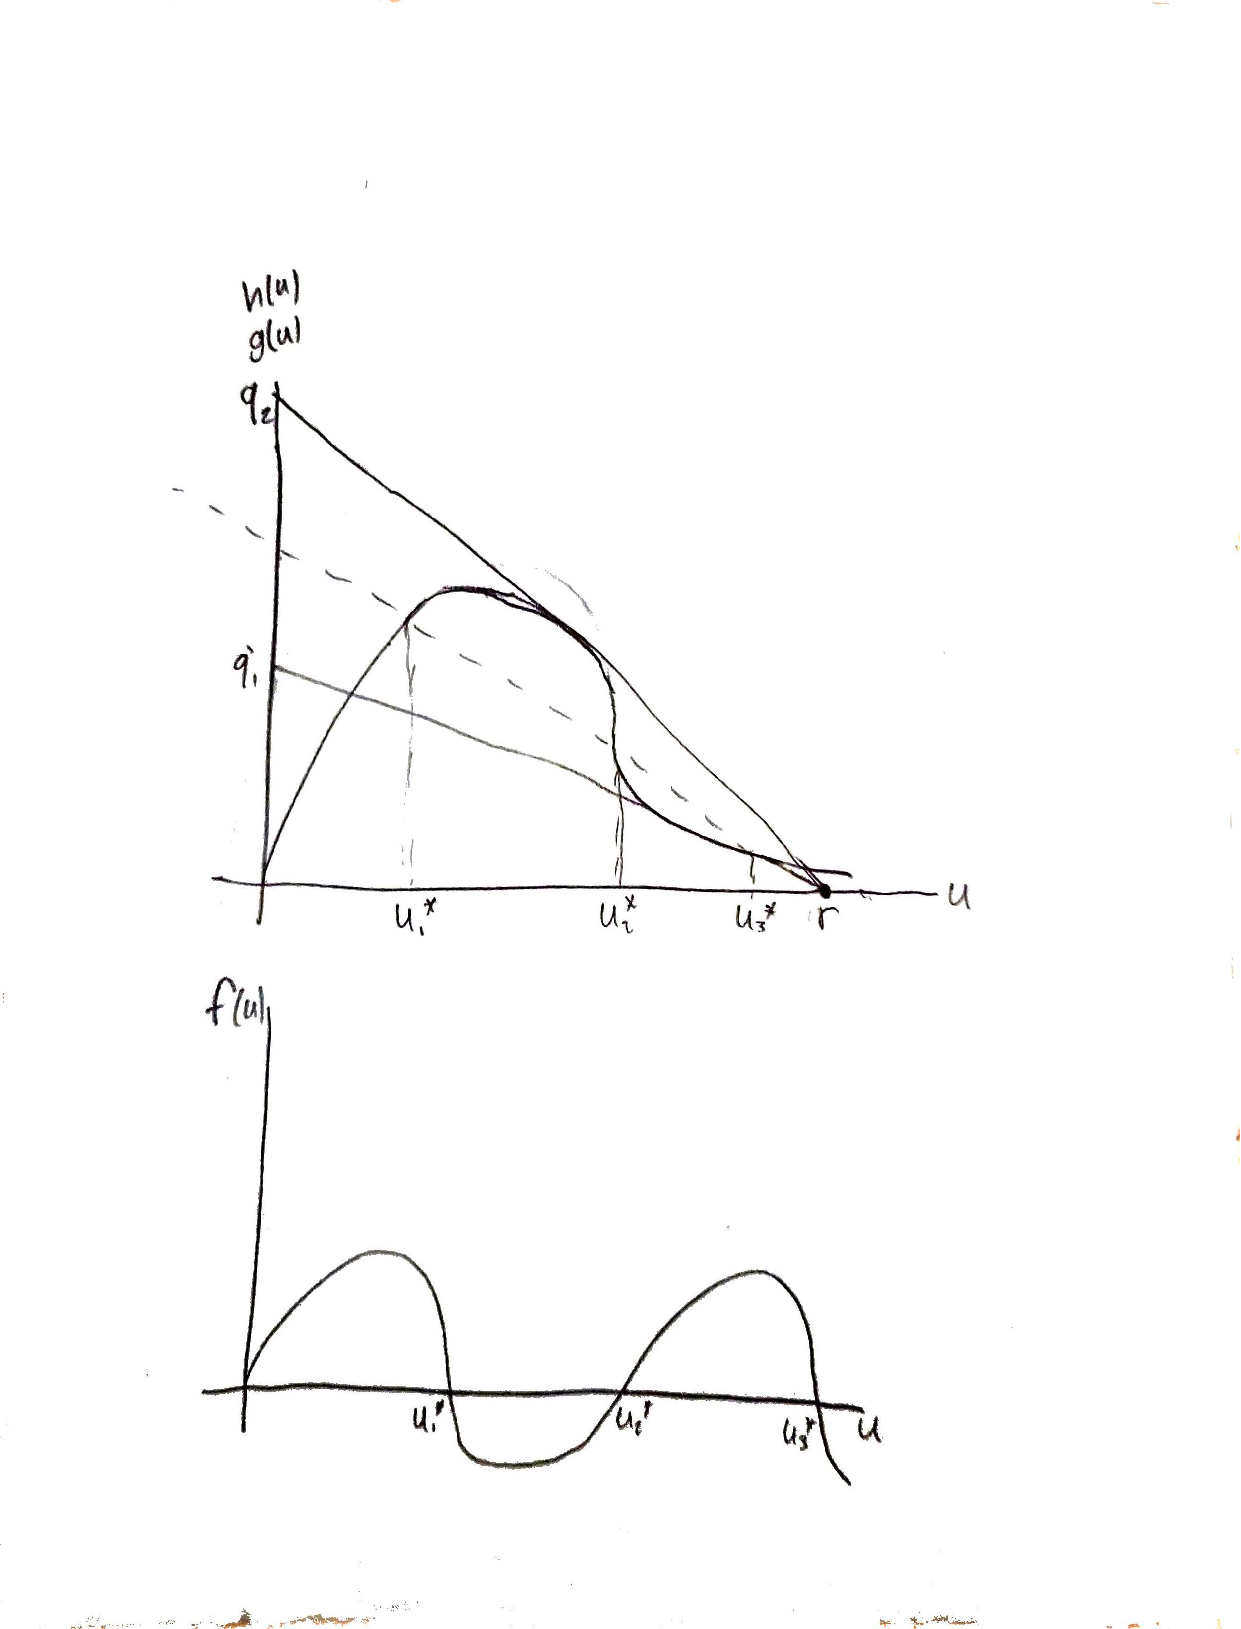
\includegraphics[width=0.8\textwidth]{Graphs1.pdf}
    \end{figure}
    Here is the bifurcation diagram and phase plot:
    \begin{figure}[H]
        \centering
        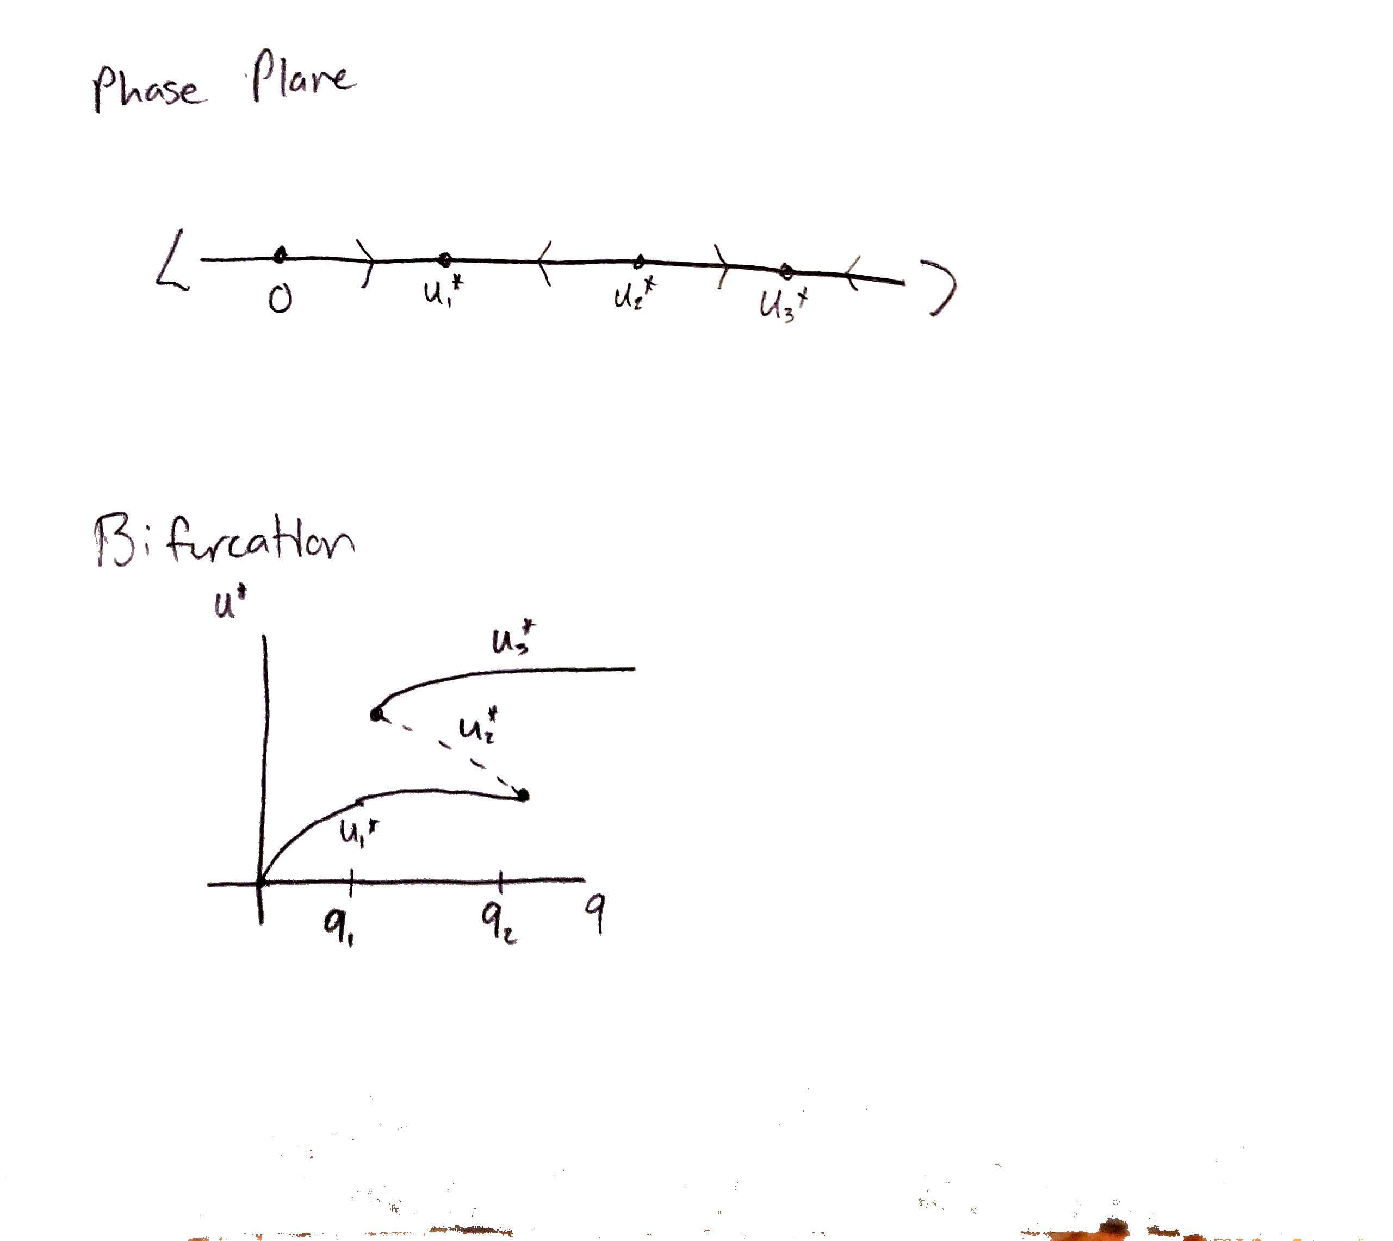
\includegraphics[width=0.8\textwidth]{Graphs2.pdf}
    \end{figure}
    \(u_1^*\) and \(u_3^*\) are asymptotically stable, and \(u_2^*\) and \(0\) are unstable.
\end{solution}


\end{document}